\subsubsection{Wookie}
\begin{samepage}
	\begin{flushright}
		\begin{tabular}{ l l }
			\textbf{Type} 			& Bipèdes \\
		   	\textbf{Planète} 		& Kashyyyk \\
		   	\textbf{Language} 		& Shyriiwook \\
		   	\textbf{Orientation} 	& Lumineux \\
		\end{tabular}
	\end{flushright}
	\vspace{-6\baselineskip}
	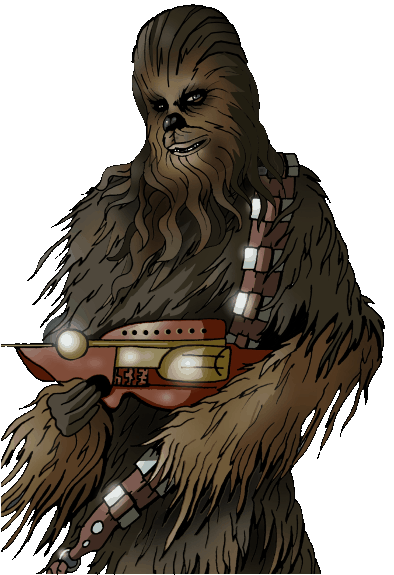
\includegraphics[width=6cm]{img/personnages/races/wookie.png}
\end{samepage}

Les Wookies sont de grand bipèdes à fourrure dépassant couramment les deux mètres de haut. Ils sont originaires de la planète Kashyyyk et n'ont que très peu de communautés en dehors de leur monde natal. Capables de vivre plusieurs siècles, les Wookies sont également dotés de longues griffes rétractiles, qu'ils utilisent principalement pour s'accrocher à la végétation dense de Kashyyyk. Leur honneur leur interdit cependant formellement d'utiliser ces griffes comme armes lors d'un combat.

\begin{description}[align=left]
\item [Force de la nature] 				% CAP +2
	L'imagerie populaire veut que les Wookies soit physiquement la race la plus forte de la galaxie (en tous cas, par rapport à sa taille).\\
	\emph{d6 For}
\item [Increvable] 						% CAP +2 +3
	Les Wookies possèdent, entres autres, de remarquables capacités de récupération, et sont capables de survivre à des blessures très graves.\\
	\emph{Increvable}\\
	\emph{Combatif}
\item [Shyriiwook] 						% CAP -1
		Les Wookies parlent entre eux leur langage, le Shyriiwook, un dialecte très complexe, en raison du mélange de feulements, rugissements, gestes et autres bruits nécessaires à son usage.\\
		\emph{Ne parle pas le Basic}
\item [Force \& Honneur] 				% CAP -2
	Comme de nombreux peuples mettant en avant des valeurs comme l'honneur, les Wookies pratiquent les serments et la "dette de vie". Celle-ci peut les amener à défendre jusqu'à la mort un étranger (même d'une autre race) auquel ils pensent devoir une grande faveur. Une dette de vie est définitive et rien ne peut la lever.\\
	\emph{Code d'honneur}
\item [Ennemis jurés] 					% CAP -1
	Les ennemis jurés des Wookies, les Trandoshans, se firent à cette époque un malin plaisir à chasser et à capturer les wookies.\\
	\emph{Ennemi Racial (Trandoshans) -4 Cha}
\item [Il faut partir à point] 			% CAP -1
	De par leur stature, les Wookies ne sont pas les êtres les plus vif de la galaxy.\\
	\emph{Allure 5}
\end{description}